\documentclass[dvips,12pt,twoside,titlepage]{article}

\usepackage[dvips]{graphicx}
\usepackage{amsfonts}
\usepackage{amsmath}
\usepackage{mychicago}
\usepackage{subfigure}
\usepackage{sidecap}
\usepackage{evolution_style}
\usepackage{xcolor}
\usepackage{float}
\usepackage[justification=raggedright]{caption}
\usepackage[subfigure]{tocloft} 
\usepackage{listings} 
\usepackage{fancyhdr}
\usepackage{rotating}
\usepackage[displaymath]{lineno}
\usepackage[flushmargin,hang,multiple,ragged]{footmisc}

\date{}

% custom commands
\raggedbottom
\setlength{\headheight}{15pt}
\renewcommand{\headrulewidth}{0pt}
\newcommand{\ud}{\mathrm{d}}
\pagestyle{fancyplain}
\cfoot{}
\lhead[\thepage]{}
\rhead[]{\thepage}
\clubpenalty=10000
\widowpenalty=10000
\renewcommand{\tablename}{\textbf{Table}}
\floatstyle{plain}
\newfloat{supfigure}{p}{sup}
\newfloat{suptable}{p}{supt}
\floatname{suptable}{Table}
\newcommand{\listsupfigurename}{List of Supporting Figures} 
\newlistof{supfigures}{supf}{\listsupfigurename}
\newcommand{\supcaption}[2]{% 
      \refstepcounter{supfigures} 
      \par\noindent\caption[#1]{#2}
      \phantomsection
      \addcontentsline{supf}{figure}{Fig. S\protect\numberline{\thesupfigures}#1}\par
}  
\renewcommand{\cftsupftitlefont}{\large\bfseries}
\newcommand{\listsuptablename}{List of Supporting Tables} 
\newlistof{suptables}{suptl}{\listsuptablename}
\newcommand{\suptcaption}[2]{% 
      \refstepcounter{suptables} 
      \par\noindent\caption[#1]{#2}
      \phantomsection
      \addcontentsline{suptl}{figure}{Table S\protect\numberline{\thesuptables}#1}\par
}  
\renewcommand{\cftsuptltitlefont}{\large\bfseries}
\DeclareCaptionLabelSeparator{emdash}{.---}
\DeclareCaptionLabelSeparator{mynewline}{\par\vspace{0.4cm}}
\DeclareCaptionLabelFormat{sformat}{#1~S#2} 
\captionsetup[figure]{labelsep=emdash,textfont=footnotesize}
\captionsetup[supfigure]{labelsep=emdash,textfont=footnotesize,labelformat=sformat}
\captionsetup[suptable]{labelsep=emdash,textfont=footnotesize,labelformat=sformat}
\captionsetup[table]{justification=centering,labelsep=mynewline}
%\newcommand{\multilineTitle}{this is the title}

\author{Kevin Bullaughey}
\renewcommand{\CorrespondingAddress}{Dept. of Ecology \& Evolution, University of Chicago \\ 
    920 E. 58th Street, CLSC 413\\ 
    Chicago, IL 60637 \\ 
    773-702-2750 (ph.)  773-834-0505 (fax)  \\ 
    \texttt{bullaugh@uchicago.edu} \vfill}
\renewcommand{\RunningHead}{Multidimensional adaptation}
\renewcommand{\CorrespondingAuthor}{Kevin Bullaughey}
\renewcommand{\KeyWords}{adaptation, natural selection, gene regulation, epistasis, models/simulations}

\begin{document}

\multilineTitle{Multidimensional adaptive evolution of a feed-forward network and\\the illusion of compensation}
 
\maketitle
\raggedright
\hyphenpenalty10000
\clearpage

\setlength{\parindent}{1cm}

\chead[K. Bullaughey]{\RunningHead}
\begin{abstract}
% BEGIN WORD COUNT
When multiple substitutions affect a trait in opposing ways, they are often assumed to be compensatory, not only with respect to the trait, but also with respect to fitness. 
This type of compensatory evolution has been suggested to underlie the evolution of protein structures and interactions, RNA secondary structures, and gene regulatory modules and networks.
The possibility for compensatory evolution results from epistasis.
Yet if epistasis is widespread, then it is also possible that the opposing substitutions are individually adaptive. 
I term this possibility an adaptive reversal.
Although possible for arbitrary phenotype-fitness mappings, it has not yet been investigated whether such epistasis is prevalent in a biologically-realistic setting.
I investigate a particular regulatory circuit, the type I coherent feed-forward loop, which is ubiquitous in natural systems and is accurately described by a simple mathematical model.
I show that such reversals are common during adaptive evolution, can result solely from the topology of the fitness landscape, and can occur even when adaptation follows a modest environmental change and the network was well adapted to the original environment.
The possibility of adaptive reversals warrants a systems perspective when interpreting substitution patterns in gene regulatory networks.
\end{abstract}

\pagebreak

\section{Introduction}

Advances in the functional annotation of DNA, combined with comparative genomic methods, allow for increasingly detailed characterizations of the evolution of biological function \cite{Andolfatto:2005p4162,Tuch:2008p1599,Gerke:2009p1558,Field:2009p4671,Chen:2010ky}.
Explanations for observed sequence changes fall into several broad categories including random genetic drift, numerous types of adaptive change, compensatory evolution, relaxation of constraint, and others.
Often several of these processes may be happening simultaneously, complicating efforts to understand the evolutionary forces behind the changes \cite{Kreitman:1996p4199,Lynch:2007if,Barrett:2011km}. 
The process of compensatory evolution is particularly compelling because it offers a means for the underlying encoding of a trait to evolve even as the correct functional output is conserved \cite{Ancel:2000p5969,Moses:2006p2892}.

Compensatory evolution has been invoked to explain the evolution of transcription factor binding sites \cite{Gibson:1996hx,Moses:2006p2892,Ludwig:2000p3921,Lusk2010}, RNA secondary structure \cite{Stephan:1996wl,Chen:1999vn,Ancel:2000p5969}, protein structure and fold stability \cite{DePristo:2005jc,Callahan:2011bk}, nucleosome positioning \cite{Kenigsberg:2010je}, and \emph{cis}/\emph{trans} interactions \cite{Landry:2005kr,Tuch:2008p1599,Kuo:2010fk}.
There are two commonly invoked modes of compensatory evolution. 
In the first, mutations are compensatory with respect to fitness, meaning that one or both of the mutations are individually deleterious, but jointly they are neutral or even advantageous. The functional effect of the alleles is not of primary relevance. 
In the second mode, the focus is the functional effect of the mutations. Jointly, the mutations preserve proper functioning of the system, but individually, one or both of the mutations would disrupt function. 
These two modes overlap when there is a direct relationship between function and fitness and often, such a relationship is implicitly assumed. 

In the case of \emph{cis}-regulatory modules, compensatory evolution is commonly offered as an explanation for functional reorganization, with nearly all such comments referring to the work of \citeN{Ludwig:2000p3921}. 
By making and expressing chimeric enhancer constructs, \citeN{Ludwig:2000p3921} showed that compensatory, epistatic changes must exist in the \emph{even-skipped} stripe 2 enhancer despite conservation of functional output. 
In this setting, it is intuitive to imagine a direct relationship between function and fitness, particularly given the expression of important developmental enhancers is most certainly under stabilizing selection, and any functional mutation would likely disrupt proper expression. 

However, when one assumes a direct link between functional changes and fitness consequences, several difficulties arise.
Even mutations of very small deleterious effect are usually eventually removed from the population \cite{Ewens:2004fj}, such that an initial deleterious substitution is unlikely and the process is likely to proceed very slowly. 
Even if compensatory evolution occurs via the joint fixation of conditionally neutral mutations, it is also likely to proceed very slowly \cite{Kimura:1985p1185,Stephan:1996wl,Iwasa:2004p1017,Durrett:2008p984}, and thus may not account for the bulk of apparent compensatory evolution. 
\citeN{Ludwig:2000p3921} had argued that nearly-neutral changes might underlie the compensatory evolution. 
This requires either very many small-effect mutations or a function-fitness mapping in which mutations of large functional effect can nonetheless be nearly neutral. This latter explanation seems plausible based on a model of enhancer function \cite{Bullaughey:2011cf}, and has been termed pseudo-compensatory change \cite{Haag:2007fu}.

While there is a tendency to assume stabilizing selection on the trait, and conclude that compensatory evolution explains turnover, adaptation is also a possibility. 
\citeN{He:2011ks} examined nucleotide substitutions in Drosophila affecting known transcription factor binding sites in developmentally-important enhancers. 
The authors characterized each substitution with respect to whether it increases or decreases the site's affinity to the transcription factor.
They found an excess of affinity-decreasing mutations in \emph{Drosophila simulans}, suggesting adaptive loss of transcription factor binding sites. 
In addition, there were some affinity-increasing mutations, but not more than expected relative to the benchmark (substitutions that did not alter affinity).
How should one interpret such changes? 
Are some of the affinity-decreasing mutations compensated by affinity-increasing mutations? 
What about the excess of affinity-decreasing mutations? 
If adaptation is really driving the loss of binding sites, how do we interpret the affinity-increasing mutations? 
Would these have been deleterious?

In answering these questions, the distinction between compensation with respect to function and compensation with respect to fitness becomes important.
Two mutations that appear compensatory with respect to function need not be compensatory with respect to fitness. 
In particular, when a system is evolving adaptively, mutations that have opposing effects with respect to a function, and thus appear compensatory, may be individually adaptive due to other epistatic changes that are occurring in the genetic background.
I term this phenomenon an adaptive reversal. 
In an adaptive reversal, the sign of the fitness effect of altering a phenotype in a particular direction flips, as changes affecting other traits occur. In this sense, it is similar to sign epistasis, in which the sign of the fitness effect of a mutation depends on the genetic background \cite{Weinreich:2005vg}.

At its simplest, epistasis is a relationship among multiple loci or traits whereby the joint effect of several changes is not the outcome expected of the individual changes (see \citeNP{Phillips:2008dm} for a good review).
Epistasis can exist for many reasons, including structural considerations, molecular interactions, relationships mediated through the concentrations of molecules (e.g., transcriptional regulation), and even host-pathogen interactions. 
Despite its obvious importance \cite{Wolf:2000vt}, we presently understand few of the seemingly infinite array of epistatic interactions, partly because it is challenging to detect \cite{Whitlock:1995vj}.
Our limited knowledge of epistasis has prompted many investigators to consider flexible models of two- or three-locus interactions, in which the epistatic effects are parameters, and not based on assumptions regarding specific biological interactions \cite{Cheverud:1996wj,Wolf:2000vt,Takahasi:2005et,Gandon:2007ip}. 
Another approach is to consider complex models that capture epistasis among many loci \cite{Gavrilets:1998dm,Weinreich:2005vg,Yukilevich:2008p593}, at many nucleotides within a locus \cite{Kauffman:1987p595,Orr:2006p805} or in many dimensions \cite{Martin:2006p1459}, but again the epistasis present in these models is not based on explicit biological mechanisms. 

One common framework for considering arbitrary epistatic relationships is the fitness landscape, with valleys and peaks representing regions of lower or higher fitness. 
Popularized early on by \citeN{Wright:1932wy}, fitness landscapes have continued to provide a fertile analogy for discussing evolutionary processes (\citeNP{Gavrilets:2004tt,SkipperJrT:2004up,Orr:2005p1460,Weinreich:2005vg}, although see \citeNP{Kaplan2008bp}). 
A fitness landscape prescribes a fitness to each multilocus genotype (or combination of phenotypes), allowing for any type of epistasis. 
The simplest fitness landscape model is Fisher's Geometrical model \cite{Fisher:1930qy}, which despite its simplicity has yielded important theoretical predictions \cite{Orr:2005p1460,Martin:2006p1459} and a framework to test empirical measurements \cite{Martin:2007p1457}. 

Yet like the models that directly prescribe epistatic interactions, most studies invoking fitness landscapes do not rely on known biological functional relationships to specify the landscape, with some notable exceptions (e.g., \citeNP{Poelwijk:2006jj,Ancel:2000p5969,Perfeito:2011fk}).
Instead, as a means of increasing generality and tractability at the cost of realism, landscapes are mainly parameterized by their dimensionality \cite{Orr:2000p3190}, covariance matrix \cite{Martin:2006p1459}, connectivity \cite{Yukilevich:2008p593,Macia:2012fx}, or degree of ruggedness \cite{Orr:2006p805}.

To evaluate whether adaptive reversals are plausible, in particular whether they stem naturally from the epistasis intrinsic to a gene network, I investigate them using an explicit model of a small regulatory network. This three-gene regulatory network, the type I coherent feed-forward loop, is a pathway that is ubiquitous in nature \cite{ShenOrr:2002jo,Mangan:2003vl}, has been well-studied in \emph{Escherichia coli}, has behavior that is accurately captured by a simple mathematical model \cite{Mangan:2003vl}, and offers an interpretable basis for fitness \cite{Dekel:2005bd}. 

\section*{Methods}

\subsection*{Dynamic model of a feed-forward gene circuit:}

A broad overview of the model and the rational is given in the Results; what follows here are the modeling details.
I closely follow the modeling conventions and notation of Alon and colleagues \cite{ShenOrr:2002jo,Alon:2006tm}, modeling network dynamics with a system of differential equations and fitness as a cost-benefit trade-off. The topology of the type I coherent feed-forward loop is given in Figure \ref{GeneCircuit}A and the network dynamics in Figure \ref{GeneCircuit}B.
The dynamics of genes $Y$ and $Z$ are modeled as a pair of differential equations:

\begin{equation*}
\frac{dY}{dt} = \beta_{y}[X^{*}] - Y \alpha_{y}
\end{equation*}

\begin{equation*}
\frac{dZ}{dt} = \beta_{z}[X^{*} \cap Y > k] - Z \alpha_{z}
\end{equation*}

\vspace{0.6cm}

\noindent $\beta_y$ and $\beta_z$ are parameters (or traits) giving the production rates of $Y$ and $Z$ respectively. In each case $X$ needs to be in its active form, $X^{*}$, and in order for $Z$ to be induced, $Y$ must be above a threshold $k$ (Iverson square brackets indicate boolean functions). The genes are degraded/diluted at rates $\alpha_y$ and $\alpha_z$, proportional to the current protein concentrations. The threshold, $k$, is an approximation to nonlinear activation dynamics of $Z$ by $Y$ \cite{Alon:2006tm}. Differential equations of this form have two solutions depending on whether production is turned on or not. For gene $Y$, the expression when the gene has been turned on for time $t$ is:

\begin{displaymath}
Y_{\mathrm{ON}}(t) = \frac{\beta_y}{\alpha_y}(1 - e^{-\alpha_y t})
\end{displaymath}

\vspace{0.6cm}

\noindent Time $t'$ after getting turned off having reached expression level $Y_{0}$, the dynamics follow an exponential decay:

\begin{displaymath}
Y_{\mathrm{OFF}}(t'|Y_{0}) = Y_{0}e^{-\alpha_y t'}
\end{displaymath}

\vspace{0.6cm}

Expression of $Z$ is similar, except that in addition to activation of $X$, $Y$ must surpass the threshold $k$ before $Z$ is expressed. This occurs at some delay, $\tau$, that is a function of the production and degradation rates associated with $Y$:

\begin{displaymath}
\tau = -\frac{1}{\alpha_y} \log(1-k\frac{\alpha_y}{\beta_y})
\end{displaymath}

\vspace{0.6cm}

Costs associated with a network may come in the form of explicit costs, such as energetic costs (i.e., transcriptional and translational costs), and in the form of implicit costs, such as the opportunity cost of deploying limited resources.
For simplicity, I assume that all these costs are proportional to the expression level of the protein with constant of proportionality, $\eta_y$, for gene $Y$ and $\eta_z$ for gene $Z$.
The cost of $Y$ for a particular signal of duration, $d$, is thus:

\begin{displaymath}
\textsc{cost}_Y(d) = \eta_y \int_{0}^{d} Y_{\mathrm{ON}}(t)\ud t + \eta_y \int_{0}^{\infty} Y_{\mathrm{OFF}}(t'|Y_{\mathrm{ON}}(d))\ud t' = \frac{\eta_y \beta_y d}{\alpha_y}
\end{displaymath}

\vspace{0.6cm}

\noindent The first term in the sum is the cost while $X$ is actively transcribing $Y$ and the second term is the cost after $X$ is deactivated and $Y$ expression is subsequently shut down. These two terms are unlikely to have the same constant, $\eta_y$, but as a first-order approximation this may not be unreasonable.

The cost of $Z$ expression is defined similarly, although upon activation of $X$, expression of $Z$ starts at a delay, $\tau$, meaning $Z$ is only expressed for a duration, $d - \tau$:

\begin{displaymath}
\textsc{cost}_Z(d) = \left\{ \begin{array}{ll}
\eta_z \int_{0}^{d-\tau} Z_{\mathrm{ON}}(t)\ud t + \eta_z \int_{0}^{\infty} Z_{\mathrm{OFF}}(t'|Z_{\mathrm{ON}}(d-\tau))\ud t' = \eta_z \beta_z \left( d - \tau \right)/\alpha_z & : \mathrm{if}\ d > \tau \\
0 & : \mathrm{if}\ d \le \tau \\
\end{array} \right.
\end{displaymath}

\vspace{0.6cm}

Similarly, I model the benefit, which captures the contribution of the network to fitness (e.g., by increasing growth rate), purely as a result of $Z$ expression and proportional to it at rate $\delta$. The benefit only applies while the signal, $S_X$ is active (i.e., when the metabolizable substrate is present), and when the signal duration is long enough for $Y$ to pass the threshold, $k$, which happens at time $\tau$:

\begin{displaymath}
\textsc{benefit}_Z(d) = \left\{ \begin{array}{ll}
\delta \int_{0}^{d-\tau} Z_{\mathrm{ON}}(t)\ud t & \mathrm{if}\ d > \tau \\
0 & \mathrm{if}\ d \le \tau \\
\end{array} \right.
\end{displaymath}

\vspace{0.6cm}

\noindent These cost-benefit assumptions are oversimplifications for several reasons. Opportunity costs likely increase faster than linearly with expression and the benefit likely shows diminishing returns \cite{Alon:2006tm}. Also, not all costs are proportional to expression, some are proportional to the production rates, $\beta_y$ and $\beta_z$; while others are proportional to the degradation rate $Y \alpha_y$ and $Z \alpha_z$. Nonetheless, these simple cost-benefit relationships capture some of the epistasis among the evolvable traits.

\subsection*{Environment-specific fitness:}

Fitness is environment-specific, with the environment entirely described by the duration distributions of true and false signals. 
I desired the false signals to be primarily short, while allowing the true signals to be substantially longer. This pattern justifies the coherent type I feed-forward network, which functions as a filter of short signals \cite{Alon:2006tm}.
I consider two environments, low- and high-noise environments.
In order to maintain a closed form for fitness, I use simple shapes for these distributions. 
The distribution of false signals, $f_{\mathrm{F}}(t)$, is quadratic in the range (0, $t_{\mathrm{F}}$) and satisfies the following criteria: 

\begin{displaymath}
f_{\mathrm{F}}(0) = 0, f_{\mathrm{F}}(t_{\mathrm{F}}) = 0, \int_0^{t_{\mathrm{F}}}f_{\mathrm{F}}(t)\ud t = 1, \textstyle t_F = \frac{1}{2}
\end{displaymath}

\vspace{0.6cm}

\noindent making $f_{\mathrm{F}}(t)$:

\begin{displaymath}
f_{\mathrm{F}}(t) = 
\begin{cases}
   \frac{6}{t_{\mathrm{F}}^2} t - \frac{6}{t_{\mathrm{F}}^3}t^2 & : \mathrm{if}\ 0 < t < t_{\mathrm{F}} \\
   0 & : \mathrm{else}
\end{cases}
\end{displaymath}

\vspace{0.6cm}

The distribution of true signals is uniform with durations spanning the range (0, $t_{\mathrm{T}}$), and also integrates to unity. Thus $f_{\mathrm{T}}(t) = \frac{1}{t_{\mathrm{T}}}$ in the interval (0, $t_{\mathrm{T}}$) and zero elsewhere. 
For a given environment, the frequency of false and true signals are $c_{\mathrm{F}}$ and $c_{\mathrm{T}}$ respectively. 
For the simulations presented, $c_{\mathrm{T}} = 0.15$.
The only difference between the low- and high-noise environments is that the abundance of false signals in the high-noise environment is $6$-fold higher ($c_{\mathrm{F}} = 0.3$) than in the low-noise environment ($c_{\mathrm{F}} = 0.05$).

The total fitness component attributable to this network motif is then the sum of two integrals over the true, $f_{\mathrm{T}}(s)$, and false, $f_{\mathrm{F}}(s)$, signal duration distributions: 

\begin{displaymath}
\textsc{fitness} = \sum_{i \in \{\mathrm{T},\mathrm{F}\}} \int_{S}c_{i}(\textsc{benefit}_Z(s)[i=\textsc{t}] - \textsc{cost}_Y(s) - \textsc{cost}_Z(s))f_{i}(s)\ud s
 - \textsc{penalty}_L - \textsc{penalty}_H
\end{displaymath}

\vspace{0.6cm}

\noindent Iverson square brackets indicate a boolean function (i.e., there is no benefit for a false signal). The penalties are introduced in order to constrain the evolvable traits from becoming too high or too low (see below). 

Putting everything together, the closed form for the fitness function, integrating over the distributions of true and false signals, is the following:
\newcommand{\aY}{\alpha_{y}}
\newcommand{\bY}{\beta_{y}}
\newcommand{\aZ}{\alpha_{z}}
\newcommand{\bZ}{\beta_{z}}
\newcommand{\nY}{\eta_{y}}
\newcommand{\nZ}{\eta_{z}}
\newcommand{\cF}{c_{\mathrm{F}}}
\newcommand{\cT}{c_{\mathrm{T}}}
\newcommand{\tF}{t_{\mathrm{F}}}
\newcommand{\tT}{t_{\mathrm{T}}}
\begin{align*}
% row 1
\textsc{fitness}&(\aY,\bY,\aZ,\bZ,k | \delta,\nY,\nZ,\cF,\cT,\tF,\tT) = \\
% row 2
& - \frac{\bY \nY (\cF \tF+\cT \tT)}{2 \aY} \\
& - \cF [\tau < \tF]\frac{\bZ \nZ}{2 \aZ \tF^3} (\tF + \tau) (\tF - \tau)^3 \\
% row 3
& - \cT [\tau < \tT] \frac{\bZ \nZ}{2 \aZ \tT} (\tT - \tau)^2 \\
% row 4
& + \cT [\tau < \tT]
 \frac{\bZ \delta}{\aZ^3 \tT} \Big(
   1 
   - \aZ \tT
   - e^{-\aZ \left(\tT-\tau\right)}
   + \aZ \tau
   + \frac{1}{2}\aZ^2 \left(\tT-\tau\right)^2
\Big) \\
& - \textsc{penalty}_L - \textsc{penalty}_H
\end{align*}
\noindent The first five parameters of $\textsc{fitness}(\cdot)$ are the evolvable traits and the remaining are for the cost and benefit functions and the signal duration distributions (see Table 1). %\ref{params}
On the right side of the equality are six terms: (i) the cost of $Y$ expression, (ii) the cost of $Z$ expression due to false signals, (iii) the cost of $Z$ expression due to true signals, (iv) the benefit due to $Z$ expression, and (v-vi) the penalties. 

\subsection*{Penalty:}

The model described thus far suffers from several unrealistic behaviors that arise when the evolvable traits reach very high or low values. There are two strategies to circumvent these problems. One strategy is to make the model more realistic, so that it captures the non-linear consequences of very small or large trait values. The alternative is to simply introduce a fitness penalty that ensures that the system will not evolve into these implausible domains. I chose the latter strategy in order to keep the model as simple as possible while avoiding unrealistic outcomes. 

As an example, the cost of protein expression should be a convex function of protein concentration \cite{Dekel:2005p1914} because, at very high expression levels, additional translated molecules deprive core cellular functions of needed protein, or become toxic. 
Rather than explicitly incorporate a non-linear cost, I achieve essentially the same constraint by penalizing high values of $\beta$. 
As another example, consider two aspects of the model: 
First, for an arbitrarily low steady-state expression level of $Y$, an appropriately small value of $k$ can be chosen to achieve any desired delay, $\tau$. 
Second, $Z$ production is independent of $Y$ expression conditional on a given $\tau$. 
These two properties lead to the unlikely behavior that $Y$ expression can be tuned to be arbitrarily low while maintaining the same profile of $Z$ expression. 
However, at very low expression levels, the concentration is no longer well-approximated by a continuous, smooth curve, and instead is highly stochastic, depending on chance molecular interactions. 
Thus, a network relying on very low expression levels to activate a downstream pathway would not reliably maintain the pathway in either the on or off state. 
This would be costly, a feature not captured by the model. 
I prevent this from occurring by penalizing very small trait values.

I chose the following arbitrary penalties for penalizing high and low values of the traits respectively:

\begin{displaymath}
\textsc{penalty}_H = \exp\Big\{\frac{1}{25}\sum_{j}q_j\Big\}
\end{displaymath}

\vspace{0.6cm}

\begin{displaymath}
\textsc{penalty}_L = \exp\Big\{-\sum_j \log(q_j)\Big\},
\end{displaymath}

\vspace{0.6cm}

\noindent where $q_j$ is the value of the $j$'th evolvable trait. 
By design, the penalty for low values is much more abrupt than the penalty for high values, reflecting the non-linearities missing from the simplified model. 
For what I consider the meaningful parameter range, these penalties have little effect on fitness, as desired. 

\subsection*{Numerical evaluation of adaptation using the small mutation size approximation:}

In order to examine whether adaptive reversals are an intrinsic result of the topology of the fitness landscape, I consider an approximation to the adaptive process that is equivalent to computing the adaptive trajectory as the mutation step size becomes infinitesimally small. 
I refer to this as the small mutation size (SMS) approximation. 

Consider the evolutionary trajectory of the population on a relatively smooth, continuous fitness landscape. 
The phenotype, $\mathbf{x} = \left(\alpha_y, \beta_y, \alpha_z, \beta_z, k\right)$, starts at coordinate $\mathbf{x_0}$ at time $t=0$, and proceeds to evolve adaptively. 
The path traced out by evolution, $\mathbf{x}(t,\mathbf{x_0})$, is thus a function of time and is dependent on the initial starting point. 
When the mutation rate is sufficiently high, and the mutational size is sufficiently small, adaptation will be nearly deterministic. 

Another interpretation of this trajectory is as an expectation, $\mathbf{\bar{x}}(t,\mathbf{x_0})$.
If the fitness landscape is sufficiently smooth, then in the current local vicinity, $\mathbf{x} + \delta \mathbf{x}$, the landscape is a hyperplane with a slope in the orientation of the gradient of the fitness function. 
The expected phenotype some time $\delta t$ in the future is simply a small step in the most up-hill direction (under the assumption of a symmetrical mutation kernel). Thus in this deterministic approximation, adaptation proceeds by marching smoothly up the landscape in the most up-hill direction.
Since future evolution in a constant environment depends only on the current phenotype and is independent of the history, one can think of the expected adaptive trajectory as satisfying a system of time-homogeneous ordinary differential equations:

\begin{displaymath}
\frac{dx_i}{dt} = h_i(\mathbf{\bar{x}}(t,\mathbf{x_0})) \qquad \forall x_i \in \{\alpha_y, \beta_y, \alpha_z, \beta_z, k\},
\end{displaymath}

\vspace{0.6cm}

\noindent where $h_i(\cdot)$ is some function of the current phenotype. Knowing each $h_i(\cdot)$ for some starting trait vector, $\mathbf{x_0}$, would then allow computation of the path using standard tools.
Note that ``time'' in the SMS approximation relates to the evaluation of the path as a system of differential equations and does not necessary correspond directly to evolutionary time.
Under the simplifying assumptions that I have described, the system of differential equations, $h_i(\cdot)$, is simply the gradient of the fitness function, $F$, evaluated at $\mathbf{\bar{x}}(t,\mathbf{x_0})$:

\begin{displaymath}
h_i(\mathbf{\bar{x}}(t,\mathbf{x_0})) = \frac{\partial F}{\partial x_i} \rule[-1.1em]{0.5pt}{2.6em}_{\ \mathbf{\bar{x}}(t,\mathbf{x_0})} \qquad \forall x_i \in \{\alpha_y, \beta_y, \alpha_z, \beta_z, k\}
\end{displaymath}

\vspace{0.6cm}

\noindent or alternatively:

\begin{displaymath}
\nabla F(\mathbf{\bar{x}}(t,\mathbf{x_0})) = \left( \frac{\partial F}{\partial \alpha_y},\frac{\partial F}{\partial \beta_y},\frac{\partial F}{\partial \alpha_z},\frac{\partial F}{\partial \beta_z},\frac{\partial F}{\partial k} \right)\rule[-1.1em]{0.5pt}{2.6em}_{\ \mathbf{\bar{x}}(t,\mathbf{x_0})}
\end{displaymath}

\vspace{0.6cm}

I perform the numerical evaluation using the classic Runge-Kutta method (RK4) for solving systems of differential equations. 
In order to ensure that numerical evaluation of the gradient-ascent path is accurate given the curvature of the surface, I shrink the move at any step of the algorithm so that it corresponds to at most a 10\% change in any single dimension.
This has the effect of limiting the rate at which a parameter changes and serves to increase the accuracy of the computed path. 

\subsection*{Adaptive walk simulations with discrete mutational effects:}

I simulate an adaptive walk using a standard technique in which candidate mutations are sampled from a mutation kernel and accepted as a substitution or rejected based on the fixation probability \cite{Gillespie:1994vr}. I compute fixation probabilities using the standard diffusion result for a haploid population \cite{Ewens:2004fj}:

\begin{displaymath}
\mathrm{Prob}(\mathrm{fix}) = \frac{1 - e^{-s}}{1 - e^{-Ns}}
\end{displaymath}

\vspace{0.6cm}

\noindent where $N = 1000$ and $s$ is the selection coefficient for the proposed mutation relative to the current fitness:

\begin{displaymath}
s = \frac{w_{\mathrm{proposed}}}{w_{\mathrm{current}}} - 1
\end{displaymath}

\vspace{0.6cm}

A mutant network is arrived at as follows. 
First a trait is chosen among the evolvable traits with equal probability; each mutation affects only a single trait. 
Second, a mutational effect size is sampled. 
I chose to represent mutations on a multiplicative scale so that effect sizes are scale-invariant; in other words, a trait always has the same probability of changing by a given fraction regardless of the current trait value.
Thus, for a mutational effect $u$ and an original trait value of $X$, the new trait value is $X' = X e^{u}$. 
Had I assumed a mutation has an additive effect drawn from a fixed distribution, then traits that evolved to large trait values would have also evolved smaller relative mutational effect sizes. 

For the simulations presented, I draw $u$ from a two-component mixture of zero-centered Gaussian distributions with $\sigma_{1} = \frac{1}{20}$ and $\sigma_{2} = \frac{1}{5}$ and mixture proportions of $0.7$ and $0.3$ respectively. 
Although arbitrary, the mutation kernel allows for a small number of large effect mutations and a larger number of relatively modest effect ones.

The adaptive walk simulations were run for 10,000 mutational proposals, resulting in an average of 24 substitutions. Given $N = 1000$, this represents a 2.4-fold increase above what would be expected under neutrality.

\section*{Results}

\subsection*{Limitations of the single gene view of adaptation:}

Consider a single gene with substitutions in its promoter on a particular lineage.
If the promoter is otherwise conserved, then the clustering of substitutions might suggest adaptation \cite{Pollard:2006bd,Holloway:2008cn,Kim:2007p5775}.
Further suppose that these substitutions are known to have sizeable functional effects.
A cartoon illustrating such a scenario (Figure \ref{GeneCartoon}) shows three substitutions that decrease and one that increases expression.
How does one interpret that one substitution is of opposite effect relative to the others?
For a single evolving trait and a constant environment, there are three basic alternatives.

The first alternative is that these substitutions are neutral with respect to fitness, despite their demonstrable functional effects. I do not further discuss this possibility, as the present study is concerned with adaptation.
In the second scenario, one mutation is deleterious and another compensatory (over-compensation is shown in Figure \ref{Horseshoe}A). 
However, only deleterious mutations of very small effect have any appreciable chance of substituting, unless the substitution occurs jointly with compensatory ones \cite{Kimura:1985p1185}, and in either case the rate of such substitutions will likely be very low \cite{Stephan:1996wl,Ewens:2004fj,Iwasa:2004p1017,Durrett:2008p984}.

In the third scenario, the functional effects are opposing, but both mutations are individually adaptive. 
Overshooting an optimum is an example of this (Figure \ref{Horseshoe}B), which requires that the curvature (or ruggedness) of the landscape be on the same scale as the mutational effect sizes. 
In the case when small mutations are more likely than larger ones (a common assumption), the overshooting alternative is less likely than simply ascending the fitness landscape.

All of the above involves consideration of only a single trait---no epistatically-interacting traits are simultaneously evolving. 
This severe assumption limits the possible interpretations of opposing substitutions that affect a single trait.
If there are epistatic interactions, more complex behaviors can arise. 
In particular, it is possible for mutations to be of opposite effect with respect to a trait but be individually adaptive (Figure \ref{Horseshoe}C). 

\subsection*{An ideal case study---the type I coherent feed-forward loop:}

In the preceding discussion, the relationships between evolvable traits and fitness were arbitrary. 
The main aim of the present study, however, is to investigate a more concrete, biologically realistic fitness landscape.
While little is known about the topology of fitness landscapes, biological systems are highly modular \cite{Hartwell:1999ef,Schlosser:2004ui,Wagner:2007hs}, suggesting progress might be made by considering a small, tractable module, the function of which is relatively well understood and isolated from the many other subsystems of the organism \cite{Alon:2006tm}. 

One such module that may be instructive is the type I coherent feed-forward loop \cite{ShenOrr:2002jo}. 
In its simplest incarnation, this small genetic network consists of only three genes (shown in Figure \ref{GeneCircuit}A). 
Gene $X$, upon responding to a signal, induces gene $Z$ both directly and indirectly via gene $Y$ with the two inputs to gene $Z$ integrated through an AND operation. 
This regulatory module occurs in many organisms including \emph{Escherichia coli}, \emph{Bacillus subtilis}, \emph{Saccharomyces cerevisiae}, \emph{Caenorhabditis elegans}, and humans (see \citeNP{Kalir:2005io} for citations), and in the best characterized regulatory network of \emph{E. coli}, it is highly over-represented \cite{ShenOrr:2002jo}.
One reason this motif may be so common is that it performs an important biological function; namely, it acts as a sign-sensitive delay element \cite{Mangan:2003vl}, in which induction of $Z$ is delayed upon activation of the signal, $S_X$, but turned off immediately upon cessation of the signal \cite{ShenOrr:2002jo}. As a result of this sign-sensitive delay, it functions to filter out short pulses in the signal, inducing whatever pathway is downstream of $Z$ only when the signal is sustained.
Figure \ref{GeneCircuit}B illustrates the temporal dynamics of this feed-forward loop. Fitness is modeled as a cost-benefit trade-off, closely following \citeN{Dekel:2005bd} and \citeN{Alon:2006tm} and motivated by optimality principles \cite{Rosen:1967ut}. In the case of the most well-studied instantiation of this motif---the \textsc{l}-arabinose utilization system of \emph{E. coli}---the benefit is primarily the ATP derived from metabolism of arabinose \cite{Mangan:2003vl}.

Finally, and importantly here, the dynamics of this network motif are well-understood and accurately captured by a simple mathematical model, and they appear accurate even when embedded in the full gene regulatory network of an organism \cite{Mangan:2003vl}. For these reasons, the type I coherent feed-forward loop is an ideal test case for adaptation in multiple dimensions, having the property that epistasis present among the functional dimensions emerges from a biologically realistic set of interactions. 

The evolutionary maintenance of this motif rather than direct regulation of $Z$ or no regulation of $Z$ may occur in a number of circumstances. 
One scenario involves a particular cost-benefit trade-off, in which there is a fixed cost of expression, independent of level, and a benefit proportional to the expression level \cite{Dekel:2005bd}. Another circumstance in which a sign-sensitive delay element will be favored is when the signal is noisy and the distribution of true and false signals differ sufficiently in their mean durations. I model this latter scenario and assume a heterogeneous mixture of true and false signals; when the signal is true, the benefit ensues, but a false signal has no benefit. When false signals are generally short, relative to true signals, this network will act as an effective filter.

\subsection*{Adaptive reversals stem directly from the fitness landscape topology:}

I investigate the prevalence of adaptive reversals using the small feed-forward network I described earlier. 
I consider only five traits to be evolvable: the degradation and production rates of $Y$ ($\alpha_y$ and $\beta_y$), the corresponding rates for $Z$ ($\alpha_z$ and $\beta_z$), and the expression threshold, $k$. I assume that each of these is continuous, which may not be a poor approximation if sufficiently many nucleotides encode each of these traits.

I first consider an idealized approximation to the adaptive process that I refer to as the small mutation size (SMS) approximation (see Methods). 
If mutations are tiny relative to the curvature of the landscape, and the mutation rate is sufficiently high, then the adaptive trajectory will track the gradient of the fitness landscape (i.e., it will climb to a local optimum via the most uphill path). 
I have formulated the fitness function in such a way that it has a closed form and known partial derivatives with respect to each evolvable trait. 
I am thus able to numerically evaluate the adaptive trajectory by taking the gradient of fitness and treating it as a system of differential equations formed by these partial derivatives, starting from some initial point in the five-dimensional parameter space. 

In this idealized adaptive process, both compensatory mutation and over-shooting the optimum are impossible, and so by projecting the adaptive trajectory onto one trait axis, any observed reversal will be a direct result of the topology and the epistasis encoded in the genetic network. 
An adaptive trajectory on this fitness landscape is a path in six dimensions---five trait dimensions and fitness. 
In order to investigate and visualize the prevalence of adaptive reversals, I computed 200 SMS adaptive paths from random starting points in the five-dimensional hypercube. Figure \ref{Traces} shows several of these trajectories projected onto two-dimensional slices of the six-dimensional fitness landscape, each slice corresponding to one evolvable trait dimension and fitness (also see Table S1 for a summary). 

There are several qualitative behaviors apparent in these projections:
(i) four of the five traits exhibit reversals, but not all traits do, 
(ii) some traits, (e.g., $k$) show much larger, more dramatic reversals than other traits, and
(iii) the reversals do not happen strictly on fitness plateaus, i.e., fitness can increase substantially even during the return portion.
Thus, even in this very low-dimensional, continuous trait setting, adaptation of some traits may often reverse course as a result of adaptive changes elsewhere.

Thus far, I considered adaptation from random starting points. However, evolution does not proceed in this way, but rather the ascent starts when a relatively well-adapted species encounters a new environment or the prevailing environment changes.

In a feed-forward loop, the major influence of the environment is the signal $S_X$, which in the case of the \textsc{l}-arabinose utilization network of \emph{E. coli}, represents the presence or absence of \textsc{l}-arabinose. I therefore define the environment by the duration distributions of true and false signals. I then consider the case of adaptation to a new environment with a higher proportion of false signals (high-noise), starting from a population well-adapted to a low-noise environment (see Figure \ref{TwoEnv}A). 

Upon introduction to the high-noise environment, the low-noise-adapted network has a much lower fitness than it had in the low-noise environment. 
In response, the network evolves towards a solution with higher fitness (Figure \ref{TwoEnv}B). 
The most pronounced reversal that occurs in this particular bout of adaptation affects trait $k$ (Figure \ref{TwoEnv}C). 
Adaptation to the high-noise environment and the reversal of trait $k$ can be interpreted as follows. In the low-noise environment, false signals were comparatively rare, and thus there was little need to delay activation of $Z$ via a high threshold $k$. 
Thus the low-noise-adapted network exhibits a low value for trait $k$. 
However, upon introduction to the high-noise environment, the most expeditious way to increase the network's fitness was to increase $k$, as this prevents $Z$ from unnecessary induction. 
As a result, $k$ quickly evolved to a higher value, and the delay in $Z$ induction, $\tau$, correspondingly increased (Figure \ref{TwoEnv}D).
However, after $\tau$ became long enough to filter out the false signals, $k$, in conjunction with $\alpha_y$ and $\beta_y$, evolved in a way that preserved $\tau$, but reduced the level of $Y$ expression, thereby lowering costs and increasing fitness. As a result, $k$ exhibited an adaptive reversal.

\subsection*{Adaptive reversals also occur with discrete mutational effects:}

While the SMS approximation is useful for showing that reversals can result solely from the topology of the fitness landscape, there are a number of unrealistic aspects to this model. First, real mutations are likely of some discrete, potentially large effect, and thus adaptation is not a smooth optimal ascent up the landscape. Second, separate biological functions are often encoded in separate locations on the DNA (e.g., \citeNP{Ptashne:1988kf,Kirchhamer:1996p4289,Barriere:2011jj}), and thus mutations may generally affect only one of the various functions.

In order to demonstrate adaptive reversals when mutational effects-sizes are discrete and affect only single traits, I simulate an adaptive walk consisting of a succession of such mutations \cite{Gillespie:1994vr}. I use rejection sampling, with the acceptance probability of a proposed mutation equal to the fixation probability (see Methods). 
In this approximation to a population process, drift and selection are both accounted for.
However, the joint fixation of mutations that would not substitute individually is not possible, removing a confounding type of compensatory change.
This modeling decision also means that linkage relationships among traits can be ignored.

In order to characterize the propensity for reversals when mutational effects are discrete, I initiate 1000 simulations from random starting points and evolve the networks in the high-noise environment of Figure \ref{TwoEnv}. 
As under the SMS approximation, adaptive reversals are common; among these simulations, there are adaptive reversals affecting 30\% of the simulations and all the traits (see Table 2). 
By dividing the adaptive reversals into two components, the initial portion and reverse portion (the portion in the opposing direction), it becomes apparent that the typical substitution on the initial portion is of much larger selective effect than the typical substitution on the reverse portion, despite that mutations on the initial and reverse portions often have similar effects on the traits (Table 2). 
This finding underscores the need to distinguish between functional effects and selective effects and it is consistent with adaptive walks on a fixed landscape offering diminishing returns \cite{Orr:2005p1460}.

Unlike in the SMS approximation, the discrete mutational effects in these simulations introduce the possibility of overshooting an optimum. To determine if this was the case for each substitution, I retrospectively assess fitness at a grid of effect sizes smaller than the observed substitution. An intervening optimum was overshot when a smaller effect size leads to a greater fitness than that associated with the observed substitution. I only count adaptive reversals that do not overshoot an intervening optimum.

As in the case of the SMS approximation, it may be more meaningful to consider adaptation to a new environment starting from a network adapted to a distinct but similar environment, rather than from arbitrary points in the fitness landscape.
Therefore, I also conduct 100 replicate simulations starting from a network that is initially well-adapted to the low-noise environment of Figure \ref{TwoEnv}, and evolve the network in the high-noise environment (all replicates start from the same point). 
Two examples, shown in Figure \ref{Simulation}, exhibit adaptive reversals affecting the production and degradation rates of $Z$ ($\alpha_{z}$ and $\beta_{z}$). 
One advantage of a model in which each substitution only affects a single trait is that the beneficial (or deleterious) effect is clearly attributable to that trait. 
In other words, substitutions that have opposite effects with respect to the trait are individually adaptive solely as a result of the mutation's effect on that trait, and not because of a pleiotropic effect of the mutation.

The replicate simulations are often very similar, as is expected when adaptation is largely determined by the topology of the landscape and when the starting point is the same for all replicates. 
Nonetheless, the replicate simulations differ in whether an adaptive reversal is observed or not.
So although adaptive reversals are observed in 70\% of the replicate simulations, others converge at near optimal solutions without exhibiting any adaptive reversals.
In this way adaptive reversals, as with many features of evolution, exhibit a high degree of stochasticity and historical contingency \cite{Lenormand:2009p1455,Bullaughey:2011cf,Salverda:2011fa}.

Traversal of a fitness landscape with discrete mutational effects is not limited to exactly ascending the fitness gradient, and thus it is even possible to have adaptive reversals involving traits that do not generally show adaptive reversals in the SMS approximation. 
For example, under the SMS approximation when starting from arbitrary parameterizations of the feed-forward network, adaptive reversals were not found to affect the production rate of $Z$, $\beta_z$ (see Figure \ref{Traces}). 
Yet in the simulations detailed in Table 2, the most commonly affected trait is $\beta_z$ and one example is shown in Figure \ref{Simulation} (right panel).
Conversely, the threshold $k$ does not show as many reversals in the discrete effect model as in the SMS approximation.
These discrepancies appear to result from the SMS approximation allowing multiple parameters to change simultaneously.
This suggests that discrete mutational effects may actually increase the opportunities for adaptive reversals.

\subsection*{Mutational target size and dimensionality:}

Adaptive reversals in the SMS approximation are impossible in one dimension, while they appear common in five dimensions (Figure \ref{Traces}). 
Clearly, the dimensionality of the landscape plays a role in whether adaptive reversals occur.
But dimensionality is not a smoothly tunable knob; instead it is the combination of particular epistatic relationships intrinsic to the network construction, dynamics, and fitness model.

In order to gain insight into whether adaptive reversals are primarily the result of epistasis between certain subsets of the traits and how the number of evolving traits affects the prevalence of adaptive reversals, I again evolved networks using the SMS approximation starting from random points. However, I constrained evolution to a subset of the evolvable traits.

I considered all 31 non-empty subsets of the five evolvable traits. 
Fixing a trait---preventing it from evolving---has several interpretations. 
First, it removes this trait and all associated epistatic interactions with other traits from the model, thereby reducing the degree of epistasis. 
Second, the fixed traits can be thought of as having a mutational target that is so much smaller than the other traits that they rarely, or in this case never, evolve.
Thus, this exercise is informative in that, in real biological systems, traits may have very different mutational target sizes, which in turn may shape which adaptive trajectories are most likely and whether adaptive reversals occur.
The results of this analysis are presented in Figure \ref{Dimension}.

As expected, adaptive reversals are absent when only one trait is allowed to evolve. 
In general, as the number of evolvable traits increases, there is a trend toward more reversals (Figure \ref{Dimension}, top) and reversals of larger effect (Figure S1). 
But this trend is not perfect; some combinations of parameters are much more likely to exhibit adaptive reversals than others. This pattern reflects the nature of the epistasis. 
For example, in landscapes with only $\beta_y$ and one other trait free to evolve, which trait exhibits reversals varies dramatically. 
When $\beta_y$ evolves in conjunction with $\alpha_y$, the former exhibits many reversals and the latter does not. 
When $\beta_y$ evolves with $\alpha_z$, the pattern is reversed, with $\beta_y$ not exhibiting many reversals while $\alpha_z$ does.
When $\beta_y$ and $k$ evolve together, both show many reversals, and when $\beta_y$ and $\beta_z$ evolve together, neither show many. 

These patterns align with the general intuition that some traits are coupled more tightly by epistatic interactions than others. 
How the propensity to undergo adaptive reversals scales to fitness landscapes of more than five dimensions remains to be seen, and will require biologically plausible higher-dimension models.

\section*{Discussion}

In principle, epistasis allows for what I call an adaptive reversal---a trait adaptively evolving in one direction and then, after a change elsewhere in the system, evolving adaptively in the reverse direction.
In such adaptive reversals, mutations of opposing functional effect are individually adaptive, which is in contrast to compensatory evolution, in which changes of opposing functional effect also have opposing fitness effects (i.e., a damaging and a restorative mutation).
Whether regulatory networks exhibit an epistatic structure that can lead to adaptive reversals is not immediately clear, however, as the epistasis is shaped by functional properties of the system.

There are a number of \emph{a priori} reasons why one might not expect adaptive reversals to be a common feature of regulatory evolution. 
First, epistasis relates to the dimensionality of the biological subsystem under consideration.
For example, epistasis internal to a protein may relate to the catalytic properties of the active domains, the shapes of the interaction surfaces, the structural scaffold, the stability of the protein, and the folding efficiency. 
The protein, in these regards, is a high-dimensional object.
In contrast, interactions in regulatory networks are largely mediated through expression levels, which are continuous and perhaps of lower dimensionality, varying only over time and space. 
Furthermore, the bulk of epistatic interactions may be among nucleotides involved in encoding a single biological function.
For example, epistasis may be common within a protein, where there may be many interacting residues \cite{Lunzer:2010co}, but less common between proteins, because interaction surfaces may be limited to a subset of domains and residues \cite{Heger:2003ts}.
Similarly, epistasis in regulatory networks may be limited by the modularity characteristic of networks \cite{Hartwell:1999ef,Alon:2003bh}; genes are encoded separately, transcriptional control is encoded separately from the determinants of transcript and protein stability, and the \emph{cis}-regulatory encoding is itself modular. 
On the other hand, in a multi-component, adaptively evolving system, adaptation may be an especially strong driver of epistatic changes in the genetic background, making the assumption of no epistasis less plausible.
So while adaptive reversals may not be surprising when one considers the dizzying possibilities for arbitrary high-dimensional fitness landscapes, that adaptive reversals occur in a relatively low-dimensional, biologically plausible model for regulatory function, is important.

In order to investigate the prevalence and nature of adaptive reversals in a setting in which the epistatic properties are determined by a biologically-plausible functional model, I employed a ubiquitous and well-understood regulatory network: the type I coherent feed-forward loop \cite{ShenOrr:2002jo,Mangan:2003vl,Alon:2007ca}. 
This network motif offers an interpretable, low-dimensional model for a component of fitness, and thus may be informative for considering the relationships among functional effects and fitness effects of mutations.
The fitness model is based on a cost-benefit trade-off relating the benefit of pathway activation and the costs associated with gene expression. 
Adaptation is generally imagined to proceed in response to environmental changes \cite{Takahata:1975ug,Gillespie:1993ww}, 
and thus by using a model with multiple environments---a low-noise environment and a high-noise environment---I was able to consider adaptation of a network that is already well-adapted to its original environment, but which can be improved by new mutations upon its introduction to a new environment. 
Considering only a modest environmental change and a network that was well-adapted to a previous environment seems more relevant than considering adaptation from an arbitrary starting point in a multi-dimensional fitness landscape, as real populations are always reasonably well-adapted to some environment, and successive environments are probably auto-correlated.
Together, the model of a small network, the cost-benefit fitness function, and the influence of the environment comprise the necessary components in order to consider whether adaptive reversals are plausible in a regulatory network.
Using this model, I have shown that substitutions that have opposing effects with respect to a trait need not be compensatory; instead there is good reason to expect such substitutions may often be individually adaptive and constitute adaptive reversals. 

There are a number of predictions based on experimental data suggesting that adaptive reversals involving protein evolution or protein-DNA co-evolution may be important. One such example involves the evolution of resistance to the antibiotic cefotaxime in \emph{Escherichia coli}. \citeN{Weinreich:2006ig} determined that 18 of the 120 possible 5-step paths that confer resistance are strictly increasing in fitness. When paths are extended to include all 18 billion acyclic paths involving reversions, only nine of these are found to be strictly increasing in fitness \cite{Depristo:2007co}. These particular paths each involve at least two adaptive reversals at the nucleotide level because the start and end sequences differ at all five considered nucleotides, and thus each site that experiences a reversion must mutate a second time. As the authors note, these nine paths are a tiny fraction of the 18 billion possible; nonetheless, these additional paths involving adaptive reversals increase by half the total number of strictly increasing adaptive trajectories. Another example involves the co-evolution of \emph{Escherichia coli} \emph{lac} repressor and its operator binding site. Using a model for fitness based in part on a large experimental dataset of reporter-operator affinities, \citeN{Poelwijk:2006jj} find that if one restricts evolution to adaptive trajectories that maintain a minimum level of affinity between repressor and operator, many of the strictly adaptive trajectories involve what they refer to as diversions, which are actually adaptive reversals at the nucleotide level. In both of these studies, adaptive reversals are at the nucleotide level, whereas in this study, I consider adaptive reversals affecting higher-order functions, and thus the constituent substitutions may be distributed among sites. 
Further progress in understanding the functional basis of adaptation should shed more light on the prevalence of adaptive reversals in a variety of systems \cite{Dean:2007ba}.

The existence of adaptive reversals has important implications for inferring the regime of selection under which a certain function or system has evolved.
Focusing on a single trait at a time rather than the system in which it is embedded could mistakenly lead one to infer the trait to be evolving under stabilizing selection (via compensatory evolution), when it is actually one component of an adaptively-evolving system.
Although it remains to be shown, the substitutions of opposing functional effect may even be helpful in detecting adaptation, when combined with data from other co-evolving traits. 
For example, when assessing whether an excess of functionally relevant substitutions have occurred on a particular lineage, rather than viewing functionally opposing substitutions as evidence of stabilizing selection on the one trait, one could incorporate them in the pool of evidence consistent with directional adaptive change of the overall system.
 
There are a number of ways in which the present model may depart from the biological reality.
First, the mutational process employed in this study operates at the level of the trait rather than at the level of the sequence. 
This property is shared by Fisher's Geometrical Model and related models \cite{Fisher:1930qy,Martin:2006p1459}. 
While this mutational process has the advantage that assumptions need not be made about the functional encoding, it implies that increases and decreases of any effect size are always possible.
For quantitative traits, these may not be unrealistic approximations \cite{hansen2006an}; however, the traits modeled here may be more granular. 
Implicit in this mutational scheme is the absence of pleiotropy.
That the production and degradation rates are separately encoded and thus not pleiotropic is likely a reasonable assumption; most regulatory elements are outside the processed transcript \cite{Maston:2006hb} and it is the transcript and resultant protein that most determine stability and degradation \cite{Ross:1996ur,Garneau:2007kq}, although exceptions to this have been recently uncovered in yeast \cite{Bregman:2011cn,Depristo:2007co,Shalem:2011eo,Trcek:2011jpa}. It is less clear whether the activation threshold, $k$, is independent from the production rate of $Y$, $\beta_y$, as these both may be encoded in the \emph{cis}-regulatory elements associated with $Y$.
Pleiotropy could also exist with traits not modeled. 
For example, the three transcription factors may participate in other regulatory circuits or have other functions, making otherwise adaptive mutations deleterious. 
Such pleiotropy can restrict the additive genetic variance available to selection and thereby limit adaptation \cite{doi:10.1146/annurev.ecolsys.110308.120232}.
Although pleiotropy is clearly biologically important, excluding it in the present study is helpful for keeping the model simple.

I also assume the environment is constant after the initial change, and although also unrealistic, it is nonetheless a common assumption when modeling adaptation \cite{Orr:2005p1460}, and it seems like a useful starting point. 
By assuming constancy of the environment, I ensure that adaptive reversals resulted from other, epistatic changes to the network, and not simply because the environment changed again.
While it is certainly possible that selective pressures change rapidly, the present study is concerned with the plausibility of adaptive reversals due solely to the fitness landscape topology.
In fully specifying the fitness function for the feed-forward loops considered, I needed to make some assumptions regarding the exact nature of the cost functions. 
Finally, in the adaptive walk simulations, I accept or reject each mutation based on the fixation probability, and thus successive substitutions are independent. 
This approach does not model certain population dynamics including the joint substitution of mutations or interference among simultaneously segregating mutations.
These dynamics are likely to be of very minor importance here, and by deliberately excluding them, I ensure that the substitutions comprising the adaptive reversal are indeed individually beneficial.

\section*{Conclusions}

I have shown how adaptive reversals can occur during the evolution of a particular regulatory motif, the type I coherent feed-forward loop.
I chose to investigate this motif because its dynamics are accurately captured by a simple mathematical model \cite{Mangan:2003vl}, it is prevalent in nature \cite{ShenOrr:2002jo,Alon:2007ca}, has an interpretable basis for fitness, and is relatively low-dimensional. 
I did not expect this particular model to have an unusual propensity to exhibit adaptive reversals.
Additional work will be needed to show whether adaptive reversals are a common feature of multidimensional evolution in other systems, and this will require appropriate, biologically-accurate models, which unfortunately remain rather few.

A necessary requirement for adaptive reversals is the existence of epistasis among beneficial mutations, which experimental data suggest may be common \cite{Weinreich:2006ig,MacLean:2010dm}. Furthermore, experimental evolution (e.g., \citeNP{Barrick:2009p1904,MacLean:2010dm}) may soon offer opportunities to test the predictions of this study. Several criteria must be met. First, the relevant pathways must be sufficiently understood and potential epistatic interactions identified. Second, the functional effects of observed substitutions must be measurable. Third, the fitness effects of individual and combinations of mutations must be measurable. Fourth, the population must evolve in an appropriate environment to drive adaptation of the pathway of interest. For select cases, all of these criteria can already be met or will likely be met imminently.

% END WORD COUNT
\section*{Acknowledgements}

I would like to thank Molly Przeworski, Bin He, Ilya Ruvinsky, Hideki Innan, Hisashi Ohtsuki, Richard Hudson, Martin Kreitman, and John Reinitz for helpful discussions. I would also like to thank Yongtao Guan, B.H. and M.P. for suggestions on the manuscript. This work was supported by a William Rainey Harper Fellowship to K.B., an NSF EAPSI and JSPS Summer Fellowship to K.B., and an HHMI Early Career award to M.P..
The author declares that he has no conflicts of interest.

\pagebreak
\normalsize

\renewcommand{\thetable}{\textbf{\arabic{table}}}
\begin{table}[p]
\caption{\textbf{Notation used for fitness function}}\label{params}
\vspace{0.3cm}
\begin{tabular}{c|p{6.5cm}|c|c|c}
\hline
\hline
               &                      & \textbf{Can}       & \textbf{Low-noise} & \textbf{High-noise} \\
\textbf{Trait} & \textbf{Description} & \textbf{Evolve} & \textbf{Optimum$^{a}$}   & \textbf{Optimum}$^{a,b}$ \\
\hline
$\aY$     & Degradation rate of gene   $Y$        & Yes & 1.31  & 0.96 \\
$\bY$     & Production rate of gene $Y$           & Yes & 1.31  & 0.68 \\
$\aZ$     & Degradation rate of gene $Z$          & Yes & 1.18  & 1.26 \\
$\bZ$     & Production rate of gene $Z$           & Yes & 45.6  & 44.5 \\
$k$       & $Y$ threshold required to express $Z$ & Yes & 0.04  & 0.16 \\
$\delta$  & Benefit per unit of $Z$               & No  & 5     & -    \\
$\nY$     & Cost per unit of $Y$                  & No  & 0.4   & -    \\
$\nZ$     & Cost per unit of $Z$                  & No  & 2     & -    \\
$\cF$     & Frequency of false signals            & No  & 0.05  & 0.3  \\
$\cT$     & Frequency of true signals             & No  & 0.15  & -    \\
$\tF$     & Maximum false signal duration         & No  & 0.5   & -    \\
$\tT$     & Maximum true signal duration          & No  & 4     & -    \\
$\tau$    & Delay before $Z$ expression$^c$       &     &       &      \\
\hline
\end{tabular}\vspace{0.2cm}\\
$^{a}$\small{For the evolvable traits, values given are those producing the highest fitness network in the given environment. For the other parameters (i.e., the non-evolvable ones), the values given define the environment and cost function.}\\
$^{b}$\small{A dash indicates that the value of the low-noise environment is also used for the high-noise environment.} \\
$^{c}$\small{$\tau$ is a function of $\aY$, $\bY$, and $k$ (see Methods).}
\end{table}
\clearpage


\renewcommand{\thetable}{\textbf{\arabic{table}}}
\begin{table}[p]
\caption{\textbf{Reversals during adaptation from random starting points with discrete-sized mutational effects}}\label{popsimTable}
\vspace{0.3cm}
\resizebox{\columnwidth}{!}{\begin{tabular}{c|c|c|c|c|c|c|c}
\hline
\hline
  & & \multicolumn{3}{c|}{\textbf{Forward portion}} & \multicolumn{3}{c}{\textbf{Reversal portion}} \\
\cline{3-8}
\textbf{Trait} & \textbf{Reversals}$^{a}$ 
  & \textbf{Steps}$^{b}$ & \textbf{median} $Ns^{c}$ & \textbf{median} $\Delta^d$ 
  & \textbf{Steps}$^{b}$ & \textbf{median} $Ns^{c}$ & \textbf{median} $\Delta^d$ \\
\hline
\hline
$\alpha_y$ &   6 & 1.0 &  94.4 & 0.567 & 4.0 & 7.1 & 1.032 \\
$\beta_y$  &  93 & 1.9 &  64.6 & 1.574 & 2.1 & 6.2 & 0.750 \\
$\alpha_z$ &  82 & 1.9 & 105.2 & 1.809 & 1.9 & 8.4 & 0.510 \\
$\beta_z$  & 136 & 1.6 & 100.4 & 1.882 & 1.7 & 9.5 & 0.527 \\
$k$        &  38 & 1.9 &  31.3 & 0.831 & 1.4 & 7.5 & 0.404 \\
\hline
\end{tabular}}\vspace{0.2cm}\\
$^{a}$\small{Reversals observed out of 1000 simulations from random starting points conditional on fitness $> 0$. Adaptation is in the high-noise environment of Figure \ref{TwoEnv}. Only certain reversals are counted: ones not including deleterious mutations, not overshooting an intervening optimum, and including substitutions with $Ns > 5$ on both initial and reverse portions.}\\
$^{b}$\small{Average number of mutations affecting the trait on the indicated portion of the adaptive reversal.}\\
$^{c}$\small{Median population selection coefficient for all substitutions affecting the trait on the indicated portion of the adaptive reversal.}\\
$^{d}$\small{Median change in the trait observed over the reversal portion, normalized by average change across all runs.}\\
\end{table}
\clearpage


\begin{figure}[p]
\begin{center}
\resizebox{0.64\columnwidth}{!}{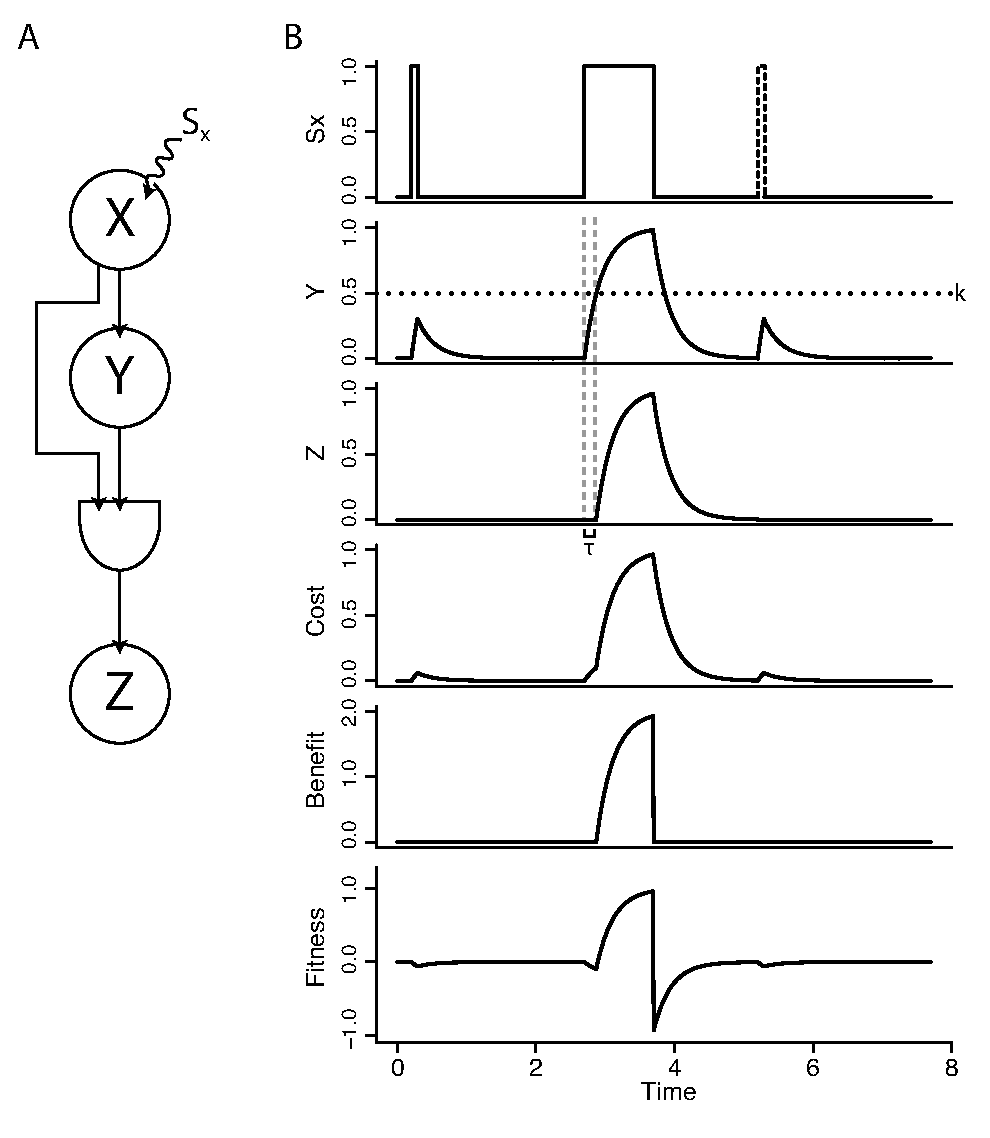
\includegraphics{eps/gene_circuit_behavior.eps}}
%GeneCircuit
\caption{Layout and dynamic behavior of a type I coherent feed-forward loop. (A) Layout of the feed-forward loop. Gene $X$ is activated by an external signal, $S_X$, and in its active state induces genes $Y$ and $Z$. Gene $Y$ also drives the expression of $Z$. The inputs to $Z$ are combined via an AND-type logical operation whereby $Z$ is only induced when $X$ is active and $Y$ is sufficiently expressed. (B) Dynamical behavior and cost-benefit basis for fitness. Each plot shows responses to three signals as a function of time (horizontal axis). Top row: There are two true signals and one false signal (dashed). Second row: Gene $Y$ is induced when $X$ is active, but it must reach a threshold $k$ before it is sufficiently expressed to activate $Z$. Third row: Gene $Z$ is only induced when $Y$ is above $k$, although at a delay $\tau$ relative to $Y$. Fourth row: Both $Y$ and $Z$ have costs proportional to their expression, with $Z$ having a much larger cost, as it encapsulates the cost of activating the pathway downstream of $Z$. Fifth row: A benefit proportional to $Z$ expression is derived from the pathway downstream of $Z$, but only in the presence of a true signal. Bottom row: The fitness rate is: benefit - cost. Total fitness (see the Methods), is an integral over time for each signal and also an integral over the signal duration distributions for true and false signals. This figure follows the illustration conventions of \protect\citeN{Alon:2006tm}, adjusted to reflect minor modeling differences.}
\label{GeneCircuit}
\end{center}
\end{figure}
\clearpage

\begin{figure}[p]
\begin{center}
\resizebox{0.50\columnwidth}{!}{
\includegraphics{eps/gene_cartoon.eps}}
%GeneCartoon
\caption{Single-gene viewpoint of nucleotide substitutions. (A) Cartoon phylogeny showing a cluster of four substitutions on a single lineage. (B) Cartoon of a gene illustrating the same four substitutions as in (A). Arrows indicate the direction of the marginal functional effect of each substitution on some aspect of gene expression. Three substitutions reduce expression and one substitution increases it. In this cartoon, all four substitutions affect regions bound by transcription factors (black boxes). Despite detailed functional knowledge, observing only this one gene in isolation without the ability to consider epistatic interactions with other genes, limits the interpretations regarding mutations of opposing functional effect.}
\label{GeneCartoon}
\end{center}
\end{figure}
\clearpage

\begin{figure}[p]
\begin{center}
\resizebox{0.95\columnwidth}{!}{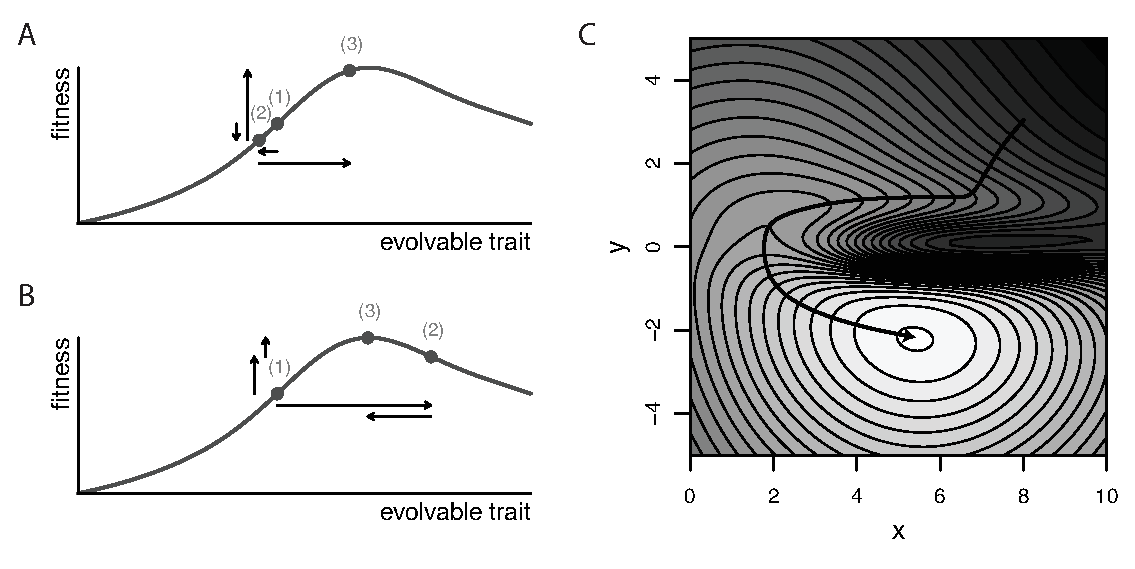
\includegraphics{eps/horseshoe_countour-with_line.eps}}
%Horseshoe
\caption{Illustration of scenarios showing how mutations of opposing functional effect can be related to smooth fitness landscapes in one (A-B) and two (C) dimensions. (A) Compensatory evolution on a fitness landscape involving one evolvable trait. Points indicate three allelic values with the starting point of the adaptive walk at {\scriptsize (1)} followed by a deleterious substitution to allele {\scriptsize (2)} and a beneficial (over-compensating) substitution to allele {\scriptsize (3)}. Horizontal arrows indicate the opposing functional changes while vertical arrows indicate the opposing changes in fitness. (B) Overshooting the optimum. Notation is as in (A), however in this example, despite opposing functional effects, the substitutions are individually adaptive. (C) Adaptation on a two-dimensional fitness landscape. Two continuous traits, $x$ and $y$, comprise the plane, while fitness is shown as a shaded topology with contour lines. The adaptive trajectory in the small mutation size (SMS) approximation, i.e., optimal hill-climbing path, is shown as the black curved arrow. Notice that with respect to trait $x$, the adaptive trajectory bends back such that initially decreasing $x$ is adaptive and later increasing $x$ is adaptive. Fitness is a carefully selected, but arbitrary function chosen for illustrative purposes: $\mathrm{fitness}(x,y) = -\frac{y}{4} + e^{-\frac{(x - 4)^2 + y^2}{50}} \Big(10 + \frac{x(1-e^y)}{1 + e^y} - 10 e^{-2y^2} (\frac{e^{-\frac{(x - 4.5)^2}{100}}}{1 + e^{4-x}})\Big)$.}
\label{Horseshoe}
\end{center}
\end{figure}
\clearpage

\begin{figure}[p]
\begin{center}
% Modified: Thu Oct 20 21:40:39 CDT 2011
\resizebox{\columnwidth}{!}{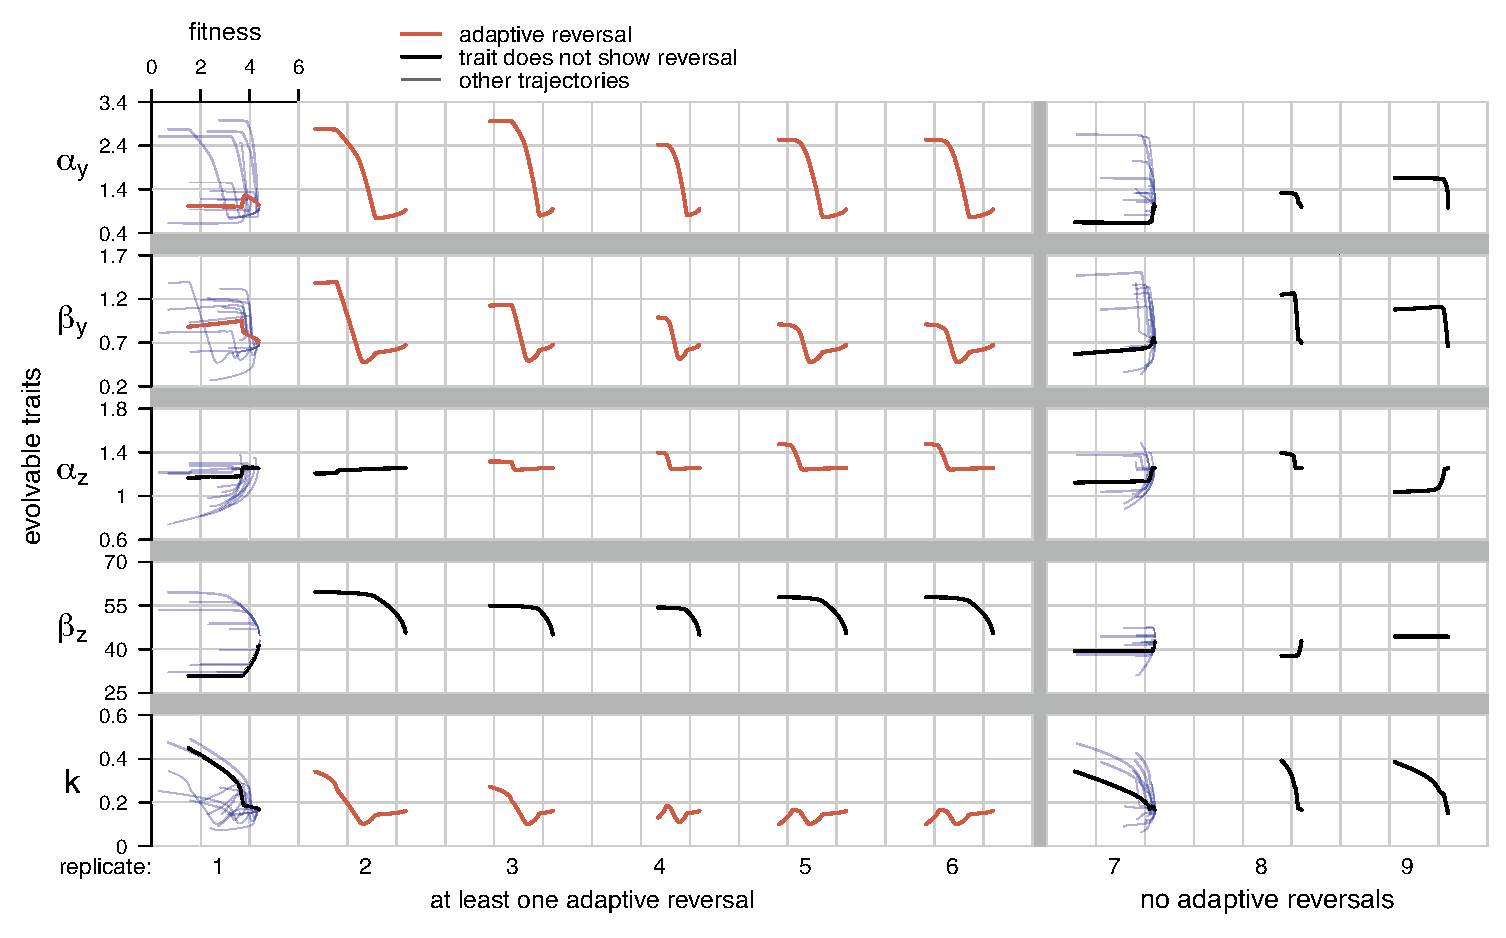
\includegraphics{eps/curves-grid-2012_05_08-fixed.eps}}
%Traces
\caption{Adaptive reversals occur solely as a result of the fitness landscape topology.
Each column highlights one adaptive trajectory (thick lines) projected onto each of the five trait dimension (rows).
The adaptive trajectory is a function of the evolvable trait (vertical axis) and fitness (horizontal axis). 
Given fitness is guaranteed to increase with time, adaptation always proceeds from left to right within each small plot.
The adaptive trajectories shown correspond to evolution starting from points sampled uniformly from a five-dimensional hypercube. Several other adaptive trajectories are shown in the background (blue lines) for replicates 1 and 7 for reference and to illustrate how adaptation always converges to the same optimal point in the fitness landscape.
The first six columns (from the left) exemplify adaptive trajectories with at least one adaptive reversal (red curves).
The last three columns show adaptive trajectories in which none of the traits undergo adaptive reversals.
All trajectories were numerically evaluated according to the small mutation size (SMS) approximation (see Methods).}
\label{Traces}
\end{center}
\end{figure}
\clearpage

\begin{figure}[p]
\begin{center}
% modified: Thu Oct 20 18:15:14 CDT 2011
\resizebox{0.9\columnwidth}{!}{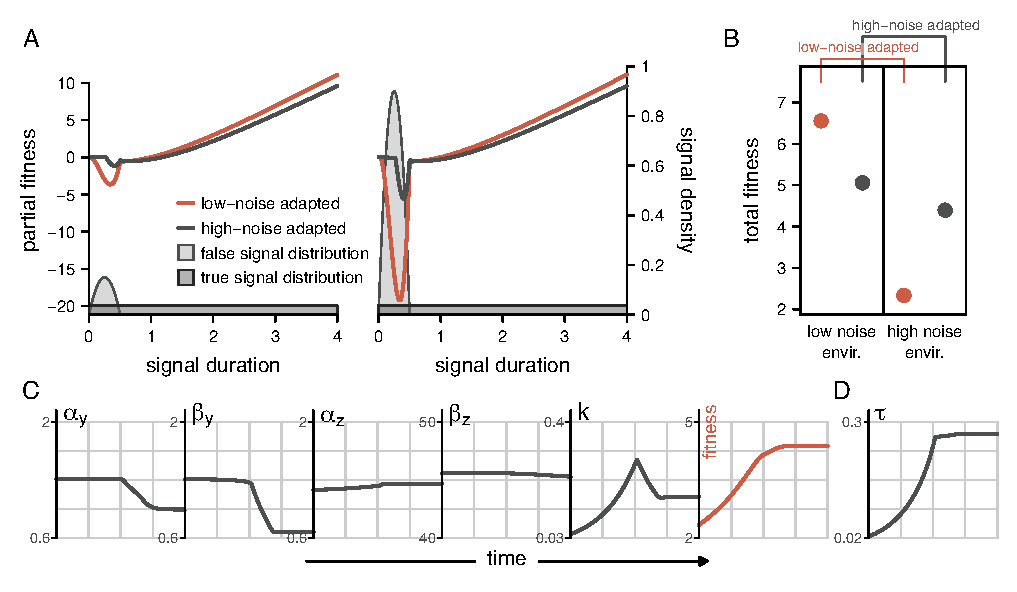
\includegraphics{eps/two_env-func_of_duration-param_limit_test-all_five.eps}}
%TwoEnv
\caption{Adaptation to a high-noise environment of a network originally adapted to a low-noise environment. (A) The two environments are defined by the signal distributions (shaded gray curves, right vertical axis). False signals are generally short (quadratic, light gray curve), with none longer than 0.5. True signals have a uniform distribution (dark gray curve).
The low-noise environment (left plot) has a much smaller density of false signals than does the high-noise environment (right plot). 
Partial fitness (left vertical axis), defined as the net fitness for a single signal, is shown as a function of the duration of the signal in each of two environments for each of two networks: the one initially adapted to the low-noise environment (red curve), and the one that evolves as a result of adaptation to the high-noise environment (gray curve). As can be seen, in the high-noise environment (right plot), the network adapted to the low-noise environment (red curve) suffers a major fitness cost for short signal durations, as these tend to be false signals, which this network fails to filter as effectively as the high-noise-adapted network. (B) Total fitnesses of each network in each environment. (C) Evolution of a trait (vertical axis) as a function of time (horizontal axis, same for each plot) for each of the five evolvable traits (first five plots). See the Methods for the interpretation of time. The sixth plot shows the increase in fitness during adaptation to the high-noise environment. (D) Evolution of the delay, $\tau$. The delay is a function of other parameters: $\tau = -\frac{1}{\alpha_y} \log(1-k\frac{\alpha_y}{\beta_y})$.}
\label{TwoEnv}
\end{center}
\end{figure}
\clearpage

%\begin{SCfigure}
%\centering
\begin{figure}
\begin{center}
\resizebox{0.80\columnwidth}{!}{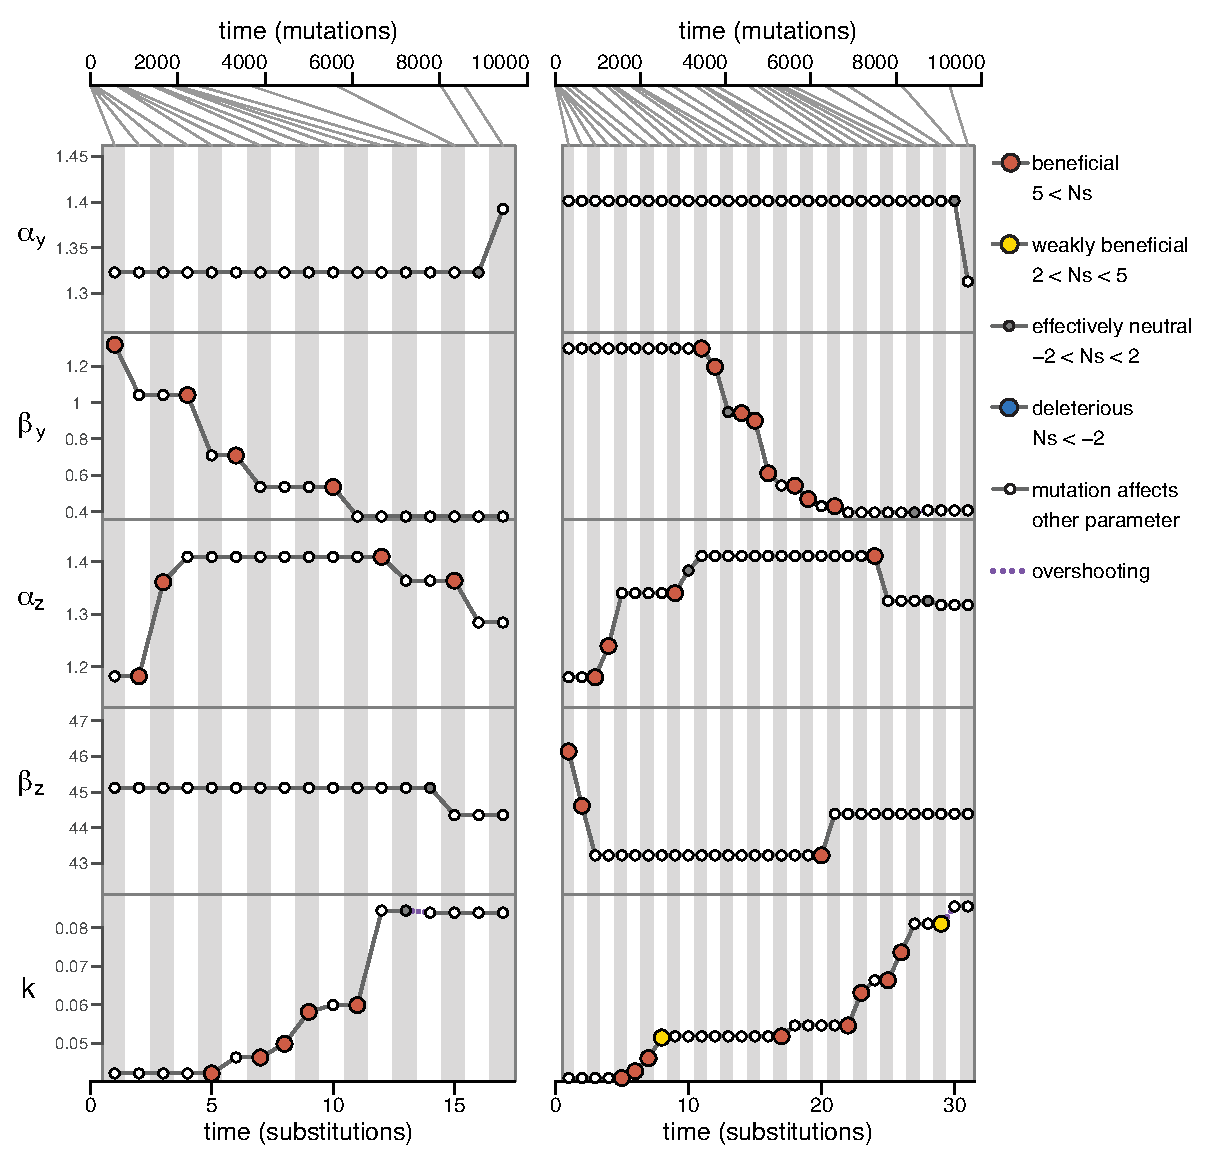
\includegraphics{eps/discrete_effects-2011_09_14-selection-two.eps}}
%Simulation
\caption{Adaptation to an environmental shift with discrete mutational effects. Two replicate bouts of adaptation are shown, starting from a network adapted to a low-noise environment, and evolving in response to a shift to a high-noise environment. Each small plot shows the evolution of one trait (vertical axes) as a function of time (horizontal axes). Vertical stripes indicate the accumulation of substitutions with the bottom axis giving the number of accumulated substitutions and the top axis indicating when the substituted mutation occurred among all mutations (most of which are lost). A mutation only affects a single trait. All substitutions are indicated on every plot, but only the colored circles correspond substitutions that affect the given trait. Thus each column features exactly one colored circle. Substitutions are colored according to the population selection coefficient, $Ns$ (see legend; $N=1000$). Purple dotted lines connecting substitutions indicate that the substitution overshot an intervening optimum. Solid lines indicate that overshooting an optimum did not occur. Adaptive reversals not overshooting an optimum can be seen in both simulations for trait $\alpha_{z}$ and in the right-hand simulation for $\beta_{z}$. \vspace{0.6cm}}
\label{Simulation}
\end{center}
\end{figure}
%\end{SCfigure}

\begin{figure}
\begin{center}
\resizebox{\columnwidth}{!}{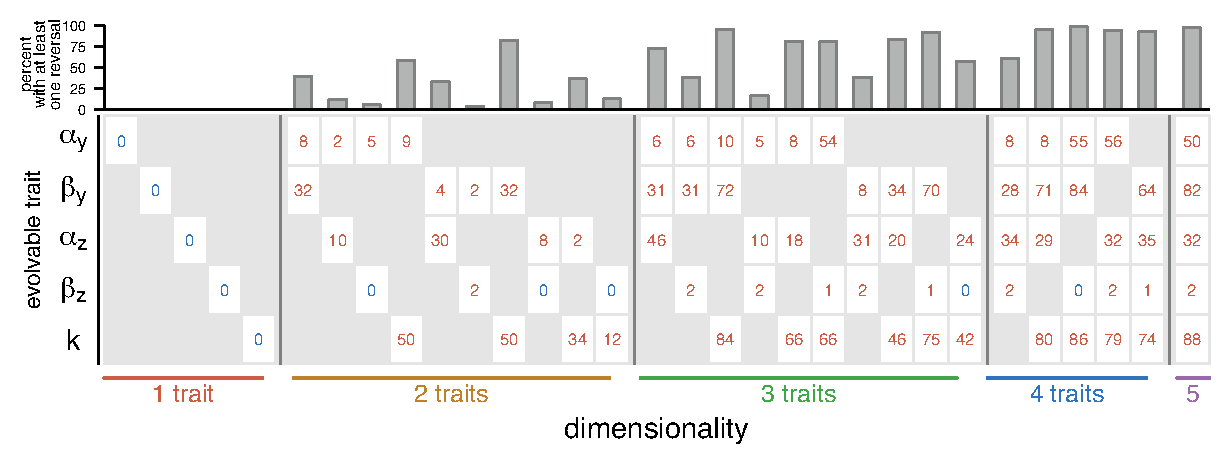
\includegraphics{eps/dimension_analysis.eps}}
%Dimension
\caption{Prevalence of reversals depends on what traits are evolvable and scales with dimensionality. 
In addition to allowing all five traits to evolve (right-most column, purple label), evolution is restricted to all possible non-empty subsets of the five traits. 
There are five possible one-trait subsets (left set, red label), ten possible two-trait subsets (second to left, orange label), and so on, arrayed along the horizontal axis. 
This allows consideration of how the prevalence of reversals scales with dimensionality or how evolution would proceed if the mutation target for one or more traits is nearly zero relative to the other traits. 
200 random starting points were sampled from the same hypercube as used in Figure \ref{Traces}. Numbers indicate percentages of adaptive trajectories showing a reversal with respect to the trait.
The fixed traits are set to the trait value that is optimal in the high noise environment. 
The bar plot above (gray bars) indicates the percentage of replicate simulations in which there is at least one reversal observed for that trait subset.
All tests for reversals are done as in Figure \ref{Traces}---the SMS gradient ascent path is computed numerically for each starting point and the high-noise environment is used.
}
\label{Dimension}
\end{center}
\end{figure}
\clearpage
\bibliographystyle{mychicago}
\bibliography{bullaughey-2012_evolution}
\end{document}

% END
